\section{Appendix: \LaTeX\xspace Tips}

\subsection{Cross References}
\label{sec:cross-ref}

Cross references are an easy way to point a reader to certain parts of the text.
For figures, tables, and equations, they are a must.
Use the \verb|\cref| command to make references to a label.
For example, if you use \verb|\label{eq:newton-second}| to label the following formula
\begin{equation}
	\vec{F} = m\vec{a}\label{eq:newton-second}
\end{equation}
you can than refer to that in the text using \verb|\cref{eq:newton-second}|.
Example: The formula in \cref{eq:newton-second} is known as Newton's second law of motion.

\subsection{Figures}

A picture says more than a thousand words.
Use \texttt{jpeg} files for photos, use \texttt{png} for screenshots, use \texttt{pdf} for everything else.
Make sure to include all text required to get a (cursory) understanding of the figure in its caption; it is no problem to have a caption spanning five lines.
Do not put a second caption in the figure itself.
For closely related content, consider using subfigures.
Draw figures yourself, but acknowledge all sources.
Check font sizes to make sure the figure is neither unreadably small nor overly big.
For example, \cref{fig:bad,fig:good} show how voltage changes over time in a bad and in a good way, respectively.
\Cref{fig:bad} is bad because you cannot read the labels on the axis, and moreover the units are missing.
What is time measured in? Seconds? Milliseconds? And voltage? Volts? Millivolts? Kilovolts?
In contrast, \cref{fig:good} is clear and easy to read.

A warm suggestion: \textbf{DO NOT} fall into the temptation of using Excel (or similar stuff) to process your data and plot your graphs.
First, it is highly inefficient: if you need to re-plot your graphs (or change the way you perform data processing) you will need to \textbf{manually change all of them!}
Second, Excel-like plots are most of the time unreadable (and ugly), and they are not suited for presenting scientific results.
Use scripts and scientific tools to process and plot your data.
For example you might use \texttt{python} with \texttt{mathplotlib}\footnote{\url{http://matplotlib.org/}}, or the \texttt{R} statistical framework\footnote{Some basic examples at \url{http://flowingdata.com/2012/12/17/getting-started-with-charts-in-r/}}, or \texttt{gnuplot}, or MatLab.

\begin{figure}[t]%
	\centering
	\subfloat[bad figure]{\label{fig:bad}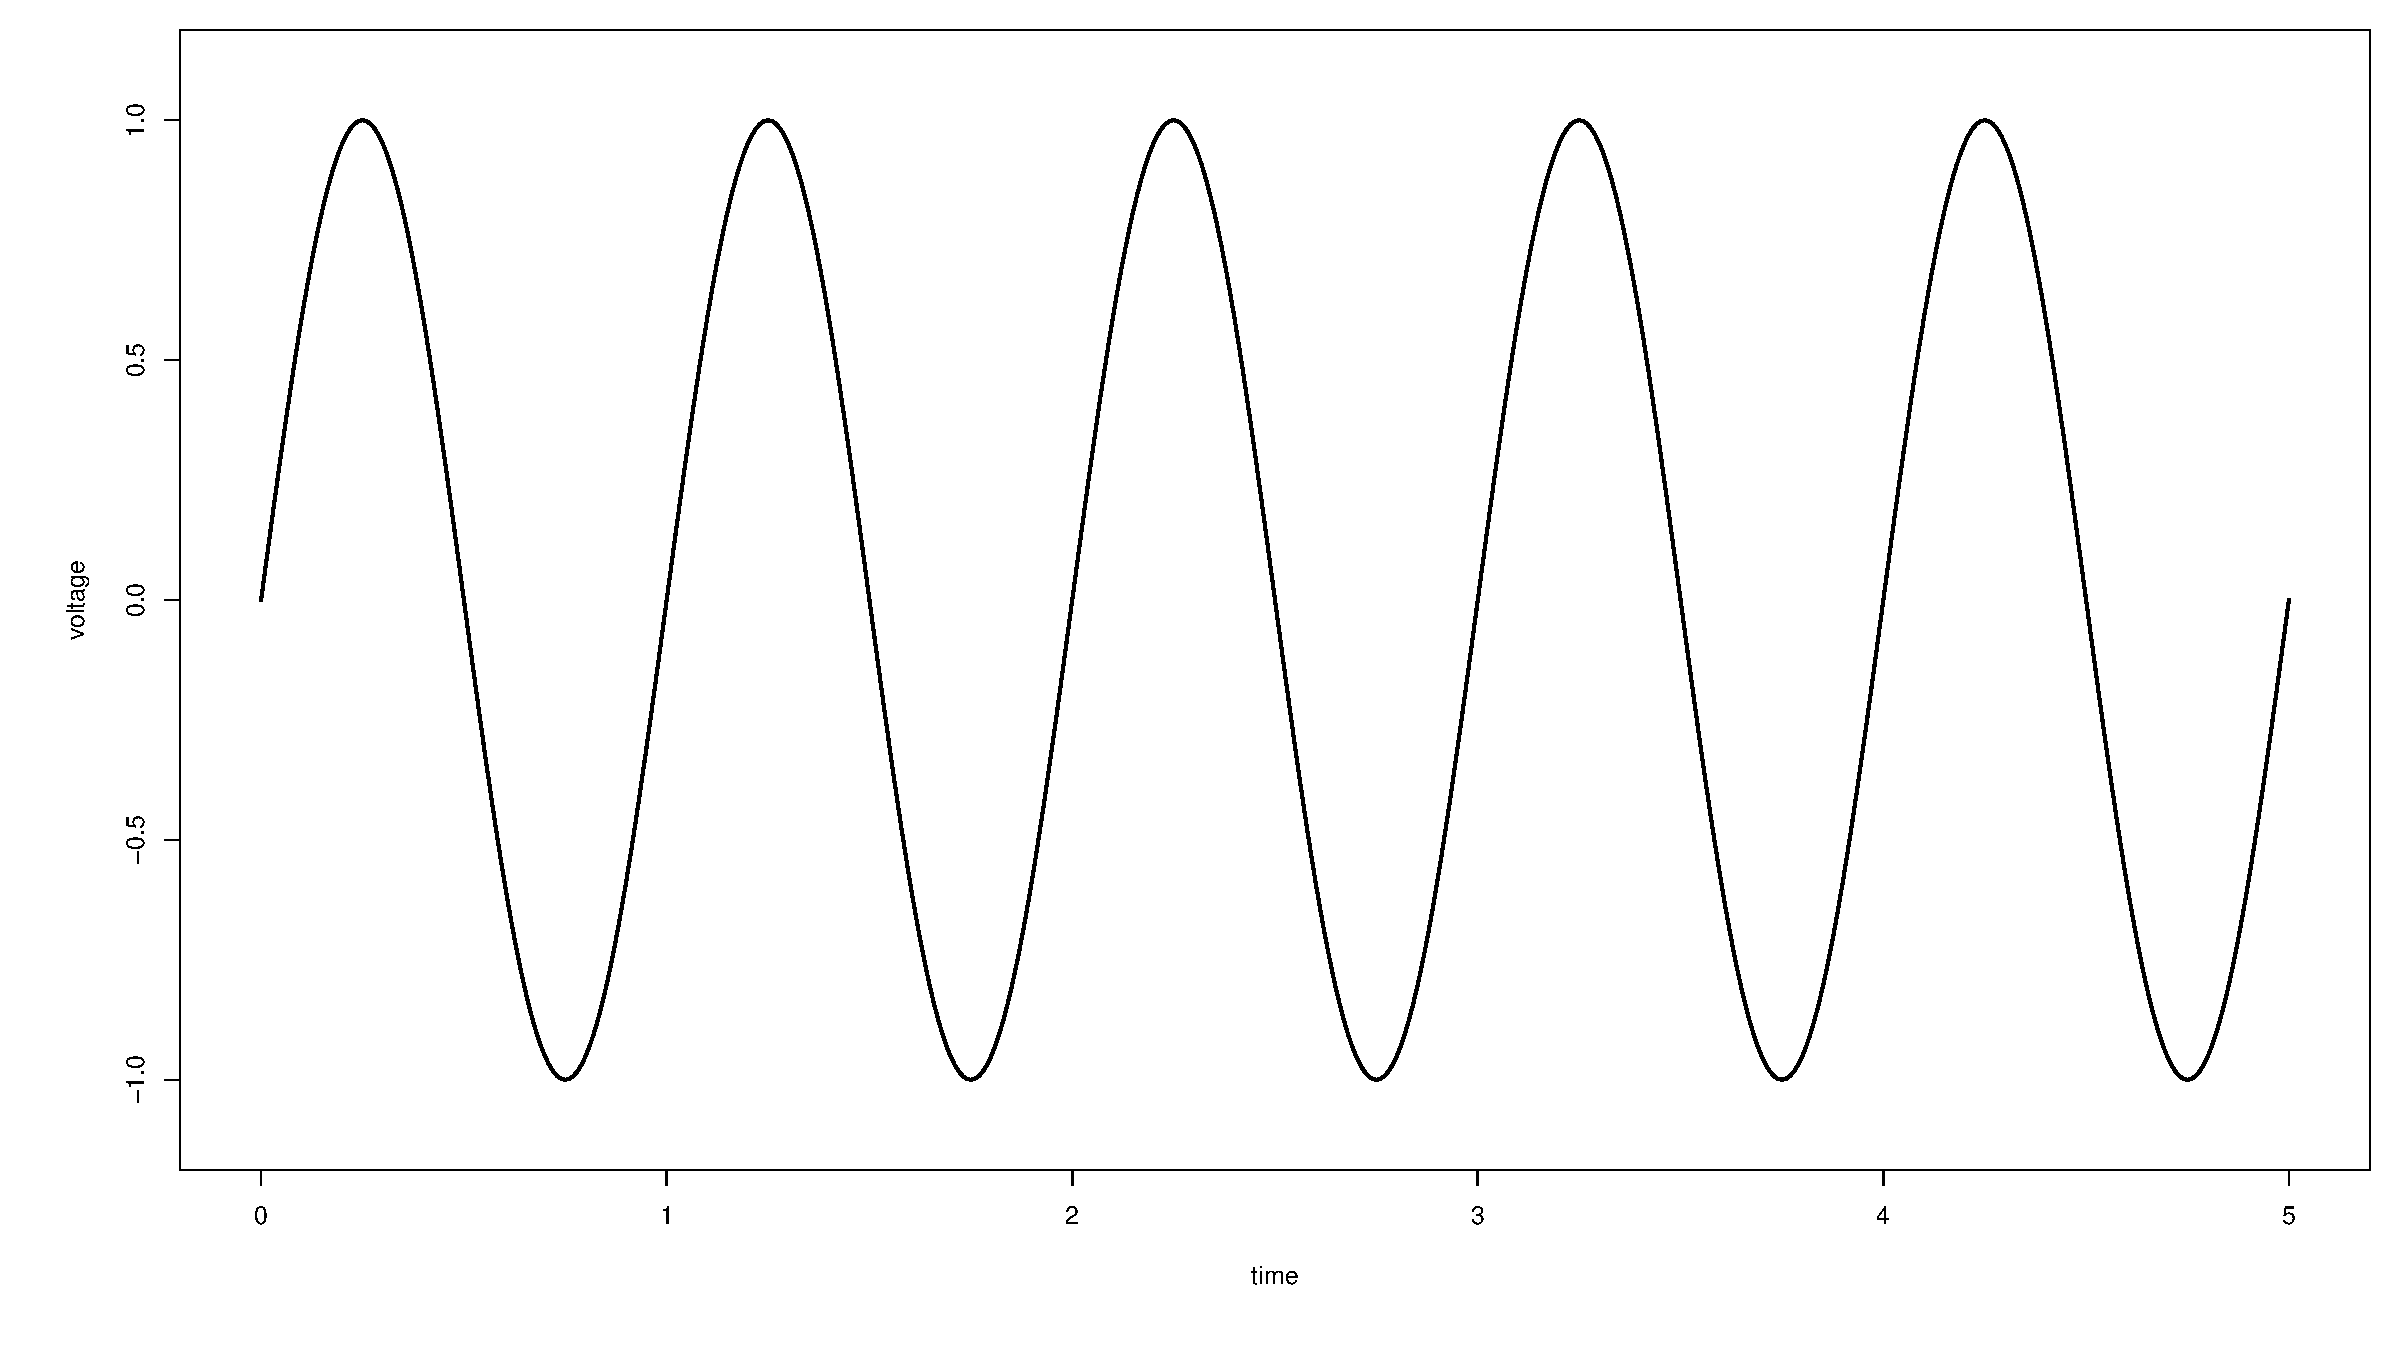
\includegraphics[width=\columnwidth]{figures/bad}}\\%
	\subfloat[good figure]{\label{fig:good}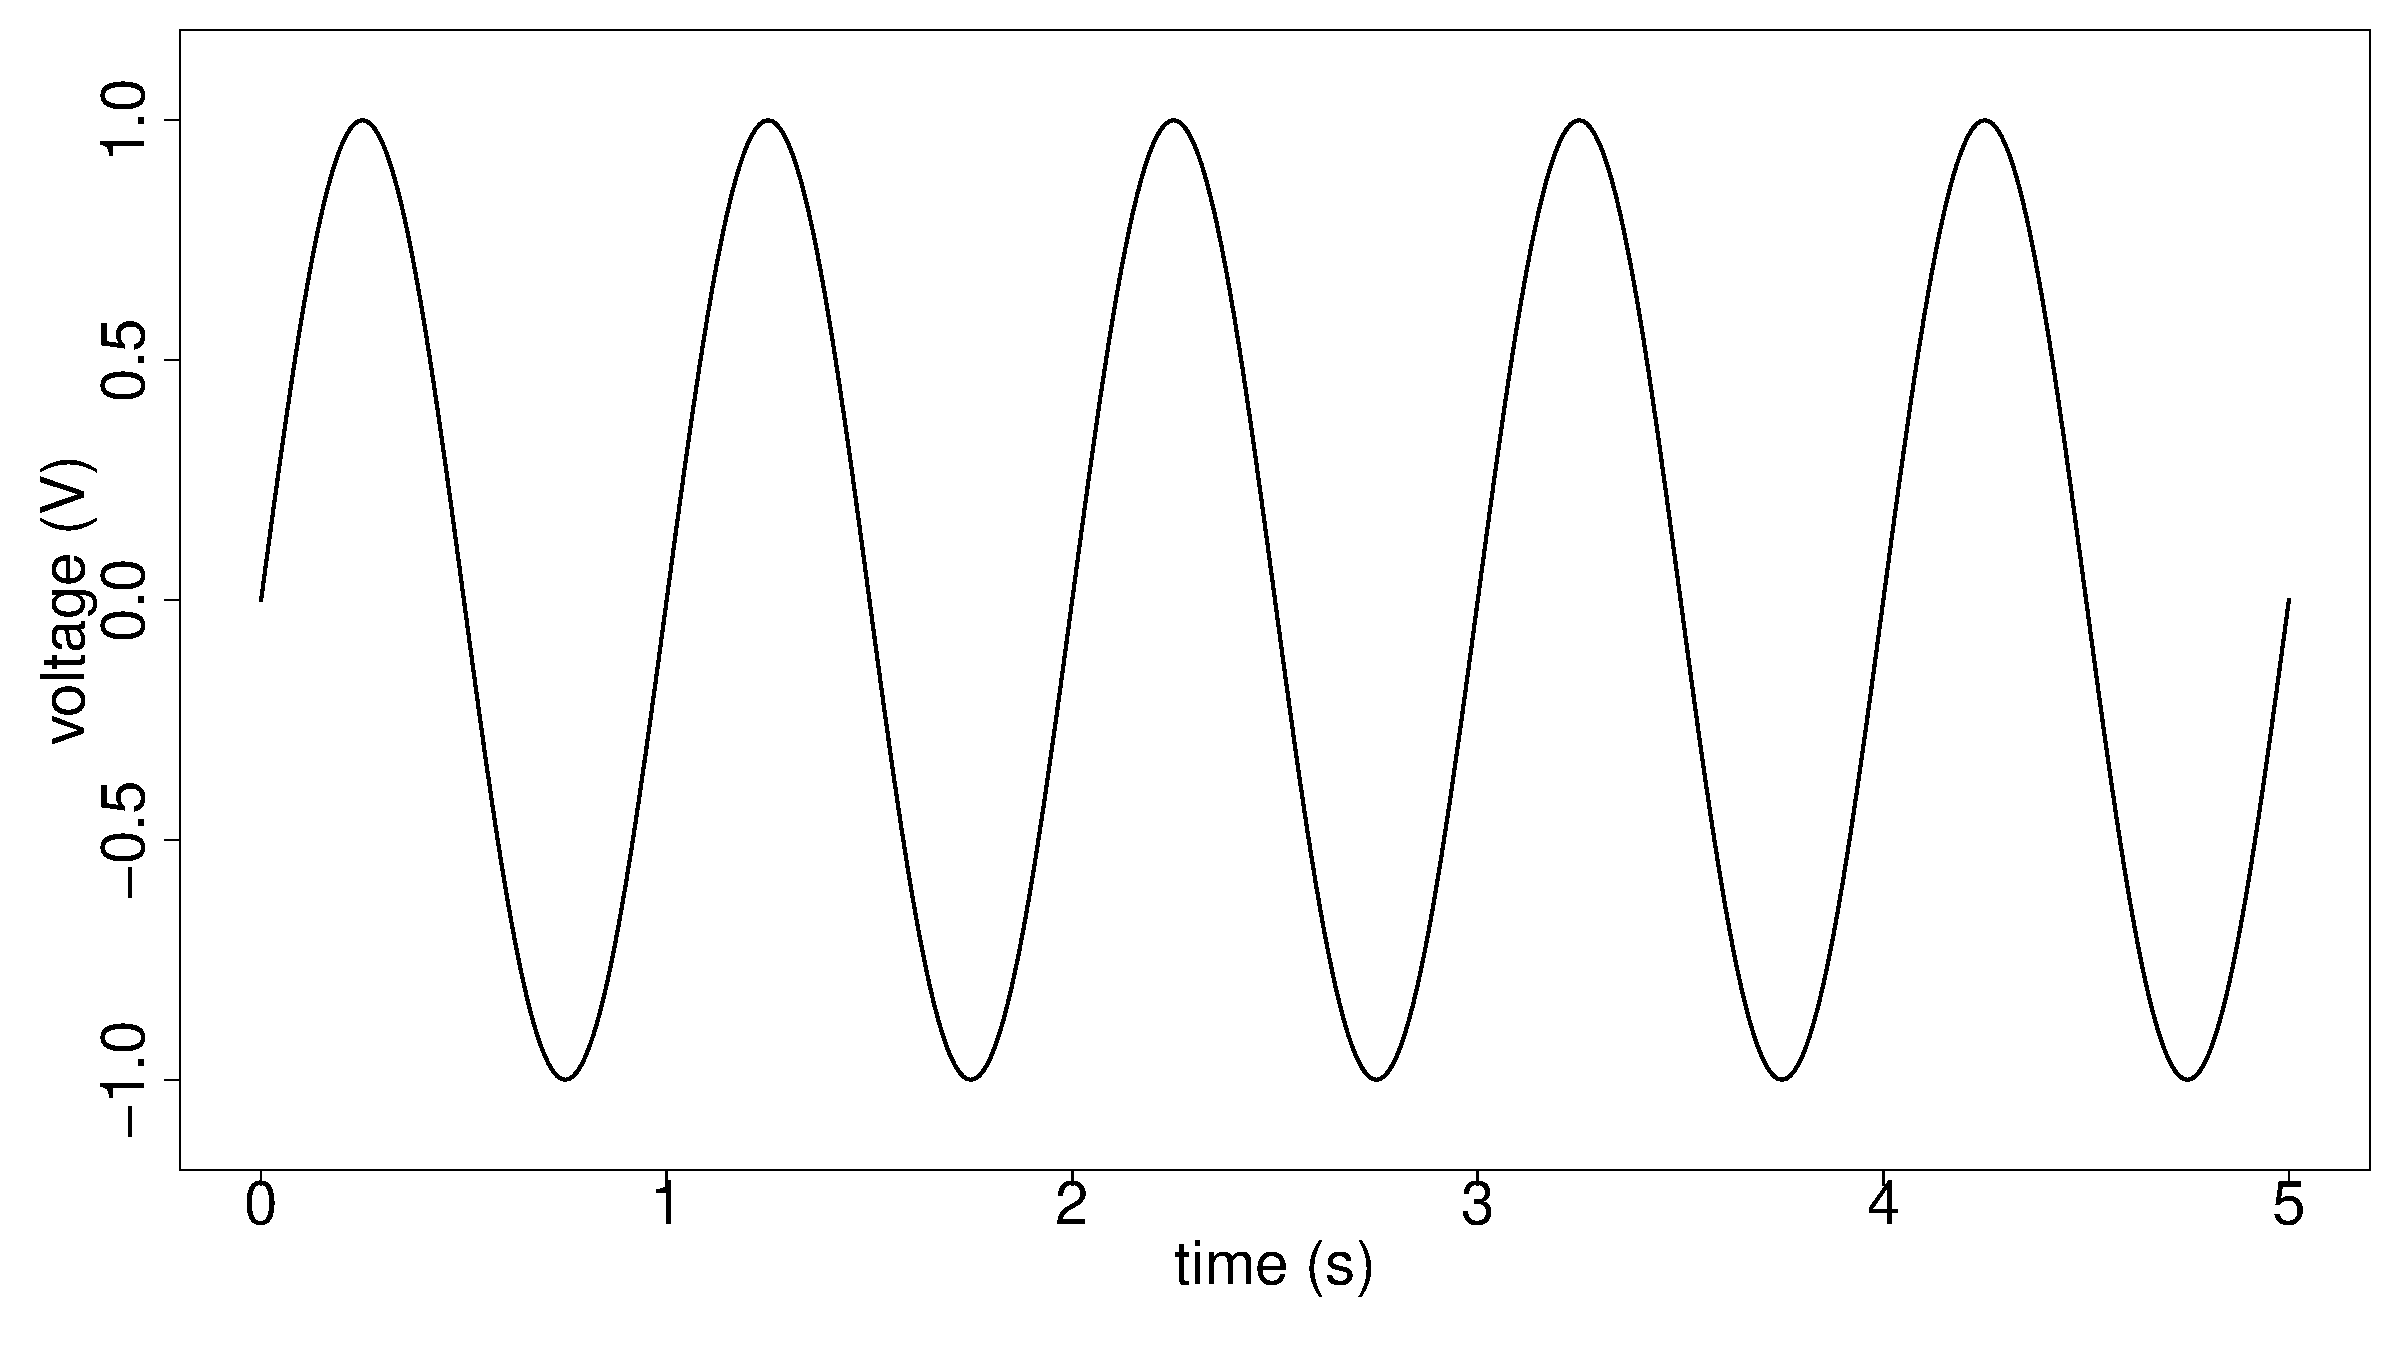
\includegraphics[width=\columnwidth]{figures/good}}
	\caption{A bad and a good representation of voltage over time.}%
	\label{fig:figures}%
\end{figure}

\subsection{Tables}

\begin{table}
	\centering
	\caption{Short table}
	\label{tab:shorttable}
	\begin{tabular}{llr}
		\toprule
		left aligned & same here & right aligned \\
		\midrule
		1 & 2 & 3 \\
		4 & 5 & 6 \\
		7 & 8 & 9 \\
		\bottomrule
	\end{tabular}
\end{table}

Use short tables, e.g., \cref{tab:shorttable} to give a brief overview of related information.
Tables are good, for example, to list your simulation parameters.

\subsection{Math}

\LaTeX's most famous feature is math typesetting.
You might need formulas for this assignment, so be sure to exploit all the power of this feature.
\begin{align}
sd_{max} &=
	\max\left(
		(t_{i+1} - t_i)
			: \zeta(t_i) < 1, i \in [0, |T|-1]
	\right)
,\\
\psi_{sd}(t) &=
	\begin{cases}
		\dfrac{\Delta t_{sd}}{sd_{max}}
			& \text{if $sd_{max} > 0$}, \\
		1
			& \text{if $sd_{max} = 0$},
	\end{cases}
\\
\zeta_{sd}(t) &= 
	\frac{
		\psi_{sd} - cl_{sd}
	}{
		c_{sd} - cl_{sd}
	}
.
\end{align}

The \emph{User's Guide for the amsmath Package}\footnote{\url{http://mirrors.ctan.org/macros/latex/required/amslatex/math/amsldoc.pdf}}, provided by the American Mathematical Society, has a comprehensive overview of best practices for typesetting mathematical content.

\subsection{Units}

Numbers with units should be set using the \verb|\SI| command, which enforces consistency throughout the text.
If you write units by your own, you will get inconsistent results: Different font faces when using text or math mode (e.g, 10 km/h versus $10 km/h$), or spacings (e.g., 10 km/h versus 10km/h), or conventions (e.g., 10 km/h versus 10 kmph).

For example: The measurements show that the car was accelerating at \SI{5}{\meter\per\second\squared} until it reached its final speed of \SI{100}{\kilo\meter\per\hour}.
Units only can be typeset using \verb|\si|; longer unitless numbers or ranges can be typeset using the \verb|\num| and \verb|\numrange| commands, respectively: The number \num{12345678} lies in the range of \numrange{10000000}{20000000}.
\Cref{tab:si-in-tables} gives an example of how to typeset numbers and units in tables.

\begin{table}
	\centering
	\caption{EMIT factors for a category 9 vehicle}
	\label{tab:si-in-tables}
	\begin{tabular}{l>{\raggedright}p{4cm}S[table-text-alignment=left,table-format=1.4e-1]s}
	\toprule
		\multicolumn{2}{l}{factor} & \multicolumn{1}{l}{value} & \multicolumn{1}{c}{unit} \\
	\midrule
		$M$ & vehicle mass & 1.3250e+3 & \kilo\gram \\
		$g$ & gravitational constant & 9.81 & \metre\per\second\squared \\
		$\vartheta$ & road grade & 0 & \degree \\
		$\alpha$ & & 1.1100 & \gram\per\second \\
		$\delta$ & & 1.9800e-6 & \gram\per\meter\cubed\second\squared \\
	\bottomrule
	\end{tabular}
\end{table}

%\section{Algorithms}
%
%Use algorithms to explain what would be too hard to express in the text body of your thesis.
%
%For example: Based on the periodically transmitted \texttt{hello} messages, the joining node gets information about its physical neighbors and their adjacent nodes.
%\Cref{alg:H_hello} depicts the handling of \texttt{hello} messages.
%
%\begin{algorithm}
%\begin{algorithmic}[1]
%\REQUIRE Locally stored state of all neighbors in set $N$
%\ENSURE Maintain neighbor set $N$ and set virtual address
%\STATE Receive neighbor information from node $N_i$
%\IF {$N_i \notin N$}
%	\STATE $N \gets N_i$
%\ELSE
%	\STATE Update $N_i \in N$
%\ENDIF
%\IF {$P==-1$ AND (Time() $-$ OldTime) $> T_{ps}$}
%	\STATE OldTime $\gets$ Time()
%	\STATE SetMyPosition()
%\ENDIF
%\end{algorithmic}
%\caption{Handle \texttt{hello} messages}
%\label{alg:H_hello}
%\end{algorithm}


%\section{Program Code}
%
%Program code should be omitted.
%What your programs do will already be explained in text form or, if needed, in algorithmic form.
%If including source code is absolutely necessary, it should be typeset as seen in \cref{lst:code}.
%
%\begin{lstlisting}[style=txt,caption=Sample application,label=lst:code]{}
%APPLICATION("printU", 192, arg)
%{
%    // Set Priority
%    NutThreadSetPriority(16);
%    // main() loop
%    for (;;) {
%        putchar('U');
%        NutSleep(125);
%    }
%}
%\end{lstlisting}

\subsection{References}

If you want to cite something proved in another work, use citations.
Search for the \texttt{bibtex} entry of the article you want to cite on \textit{ieeexplore} or \textit{google scholar}.
Put your \texttt{bibtex} code into \texttt{references.bib} and cite them using the \verb|\cite| command.
For example: According to \cite{akyildiz2002survey}, $1 + 1 = 2$.
The entries you cite will \textbf{automatically} appear in your references.

When citing more than a few pages worth of text, point the reader to the specific part you are referring to in your citation, like so:~\cite[Table IV]{dietrich2009lifetime}.

Do not cite URLs. For pointing a reader to interesting websites, use footnotes.

\subsection{Abbreviations}

Abbreviations should be explained when first used.
Latex helps by providing an \verb|\ac| command that will automatically expand an abbreviation on first use.

Example: \acp{MANET} have been frequently used as examples for the development of \ac{WSN} applications.
The literature provides hundreds different proposals of routing protocols for \acp{MANET}.
\subsection{Tips for Compiling your Latex Document}

Manually compiling your Latex document every time you make a change is terribly annoying.
Latex comes with a script which monitors your files and automatically re-compiles your document whenever a change in the file occurs.
If you change your text, you substitute a picture, or change your references, the script will re-build the pdf.

To use \texttt{latexmk}, first create (or edit) the \texttt{.latexmkrc} file in your home folder, independently from the OS (Linux, OS X, or Windows).
Inside the file put the following:

{\footnotesize
\begin{verbatim}
$pdflatex = 'pdflatex -interaction=nonstopmode';
\end{verbatim}
}

This will avoid \texttt{pdflatex} to stop in case of errors.
Then add the following (depending on your operating system and your pdf viewer).

On Linux

{\footnotesize
\begin{verbatim}
	$pdf_previewer = "start evince 2>/dev/null";
\end{verbatim}
}
On Mac OS X

{\footnotesize
\begin{verbatim}
	$pdf_previewer = "open ";
\end{verbatim}
}
On Windows

{\footnotesize
\begin{verbatim}
	$pdf_previewer = 'start "c:/Program Files\
	    /SumatraPDF (x86)/SumatraPDF.exe" %O %S';
\end{verbatim}
}

Then open your terminal, \verb|cd| into the folder where you have your latex document, and type

{\footnotesize
\begin{verbatim}
	latexmk -pdf -pvc <your-document-name.tex>
\end{verbatim}
}

On Windows you might need to type \verb|latexmk.exe|.
The script will compile your pdf and open the viewer when done.
If you make any change to your document and save it, you will see the script re-compiling the pdf.
The viewer should also automatically refresh the pdf.

\subsection{Concluding Remarks}

When working with latex, remember that this tool has a computer-science-like philosophy.
Everything is done \textbf{automatically}.
If you need to do something manually, you are doing something wrong!
You just want to write your text and let your computer do all the boring stuff (numbering pictures, link cross-references, list bibliography entries, align equations, \dots).
Remember to work smarter, not harder!
If you have troubles you cannot solve by browsing through the Internet, write us.

Good luck with your work!
